\documentclass[usenames,dvipsnames]{beamer}

\mode<presentation> {
\usetheme{Montpellier}
}

\usepackage{graphicx} % Allows including images
\usepackage{booktabs} % Allows the use of \toprule, \midrule and \bottomrule in tables
\usepackage[frenchb]{babel}
\usepackage[T1]{fontenc}
\usepackage[utf8]{inputenc}
\usepackage{algorithm2e}
\setcounter{tocdepth}{2}
\graphicspath{{../../Figures/}}

\DeclareMathOperator*{\argmin}{arg\,min}
\DeclareMathOperator*{\argmax}{arg\,max}
\newtheorem*{proposition}{Proposition}
\newcommand\Fontvi{\fontsize{8}{8}\selectfont}

% exercices comptés
\newcounter{numexos}%Création d'un compteur qui s'appelle numexos
\setcounter{numexos}{0}%initialisation du compteur
\newcommand{\exercice}[1]{%Création d'une macro ayant un paramètre
\addtocounter{numexos}{1}%chaque fois que cette macro est appelée, elle ajoute 1 au compteur numexos
\textcolor{DarkOrchid}{Exercice\,\thenumexos\,:}\,#1%Met en rouge Exercice et la valeur du compteur appelée par \thenumeexos
}

\setbeamertemplate{title page}{
    \centering

    \Large\bfseries
    Machine learning Tek 5: simplicity bias of neural networks

\begin{figure}[!h]
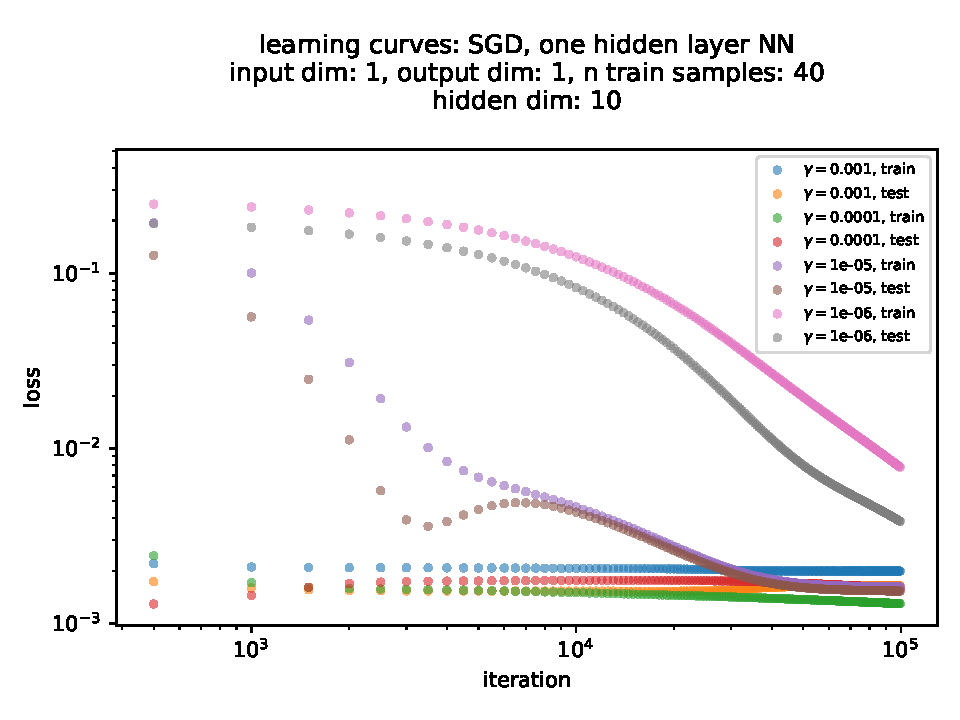
\includegraphics[width=8cm]{learning_rates_dim_h_10}
\end{figure}

    }

\title[FTML]{title}


\date{} % Date, can be changed to a custom date

\makeatletter
\let\@@magyar@captionfix\relax
\makeatother

\begin{document}

\begin{frame}
\titlepage % Print the title page as the first slide
\end{frame}

\section*{Introduction} % (fold)
\label{sec:section_name}

\begin{frame}
\frametitle{} % Table of contents slide, comment this block out to remove it
\tableofcontents % Throughout your presentation, if you choose to use \section{} and \subsection{} commands, these will automatically be printed on this slide as an overview of your presentation
\end{frame}

\section{Data}%
\label{sec:Simplicity bias}

We will perform regression on this data:

\begin{figure}[htpb]
	\centering
	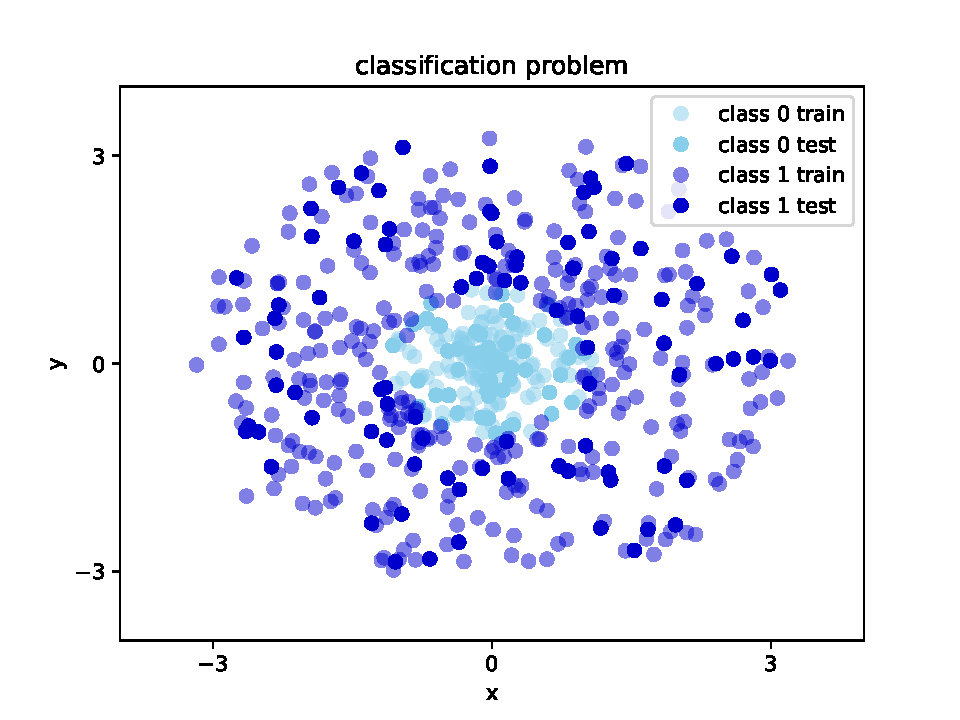
\includegraphics[width=0.8\textwidth]{data}
	\caption{data}
	\label{fig:data}
\end{figure}

\section{Polynomial regression and overfitting}%
\label{sec:Polynomial regression and overfitting}


\begin{frame}{}
We have seen that polynomial regression without regularization can \textbf{overfit}:

\begin{figure}[htpb]
	\centering
	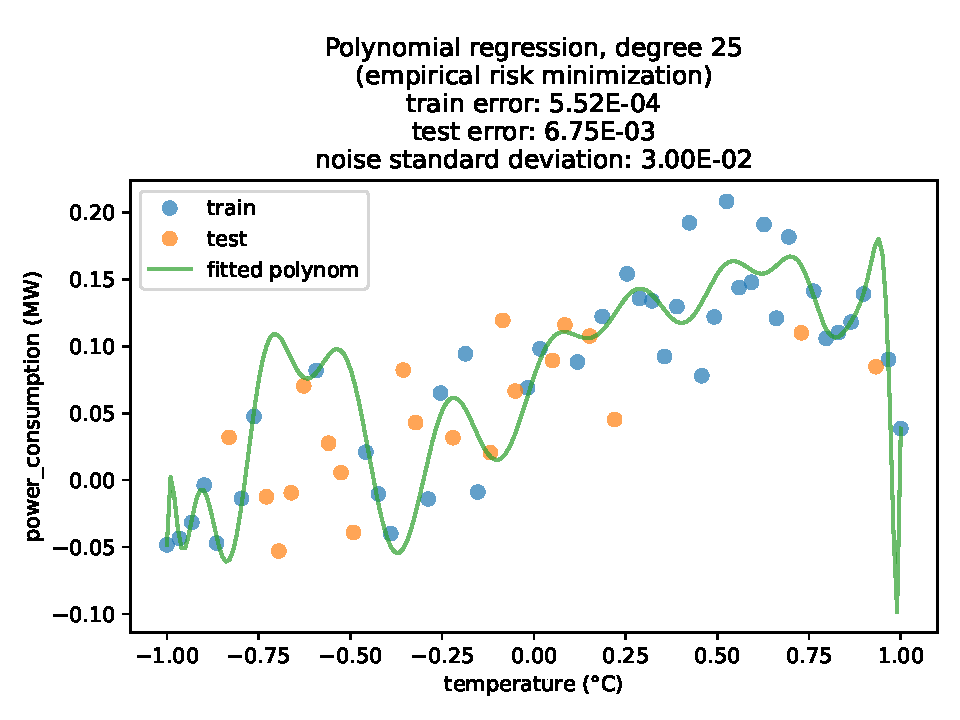
\includegraphics[width=0.7\textwidth]{polyomial_regression_std_3_00E-02_degree_25}
	\caption{Overfitting of a neural network with 26 parameters}
	\label{fig:polyomial_regression_std_3_00E-02_degree_25}
\end{figure}
\end{frame}

\begin{frame}{}
\begin{figure}[htpb]
	\centering
	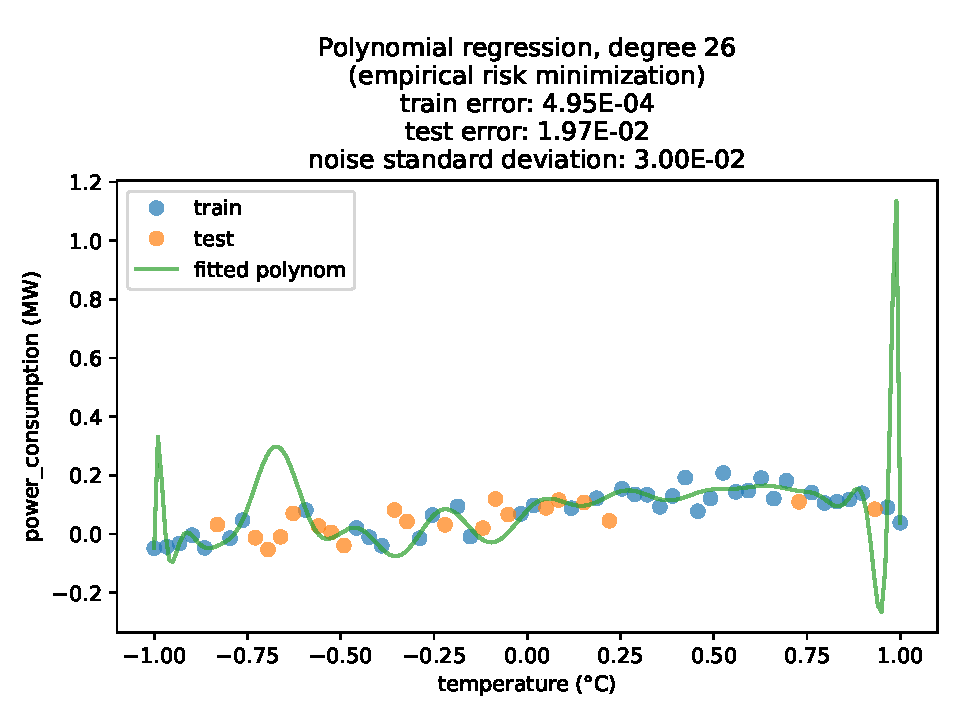
\includegraphics[width=0.8\textwidth]{polyomial_regression_std_3_00E-02_degree_26}
	\caption{Overfitting of a neural network with 27 parameters}
	\label{fig:polyomial_regression_std_3_00E-02_degree_25}
\end{figure}
\end{frame}

\begin{frame}{}

    \begin{figure}[htpb]
    	\centering
    	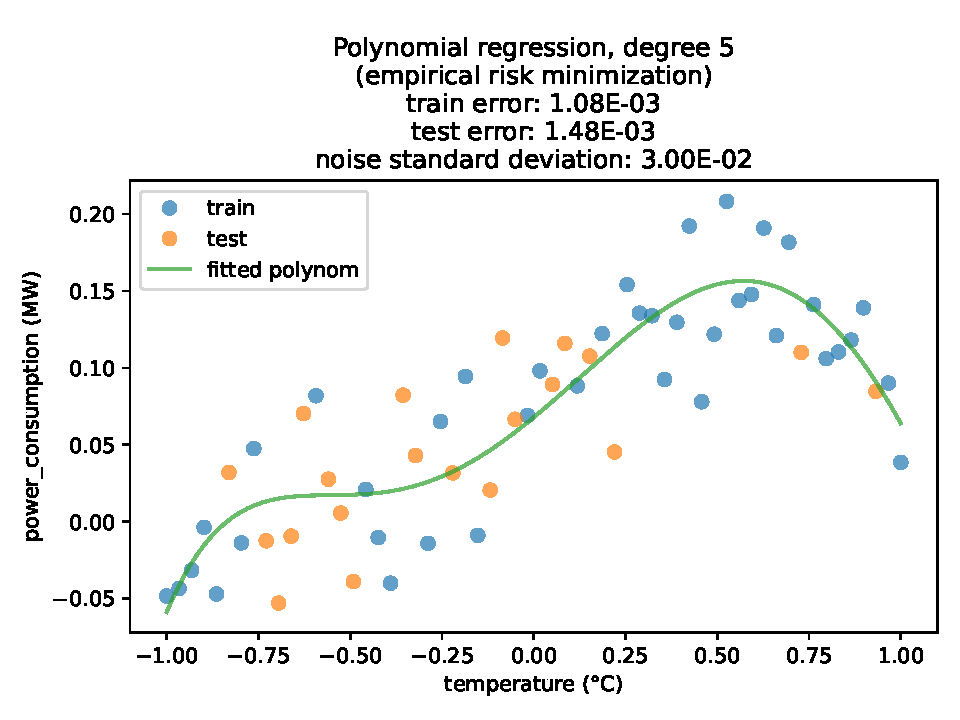
\includegraphics[width=0.8\textwidth]{polyomial_regression_std_3_00E-02_degree_5}
    	\caption{With only $6$ parameters, polynomial regression does not overfit.}
    	\label{fig:}
    \end{figure}

\end{frame}

\section{Neural network regression}%
\label{sec:Neural network regression}

\begin{frame}{}
\begin{figure}[htpb]
	\centering
	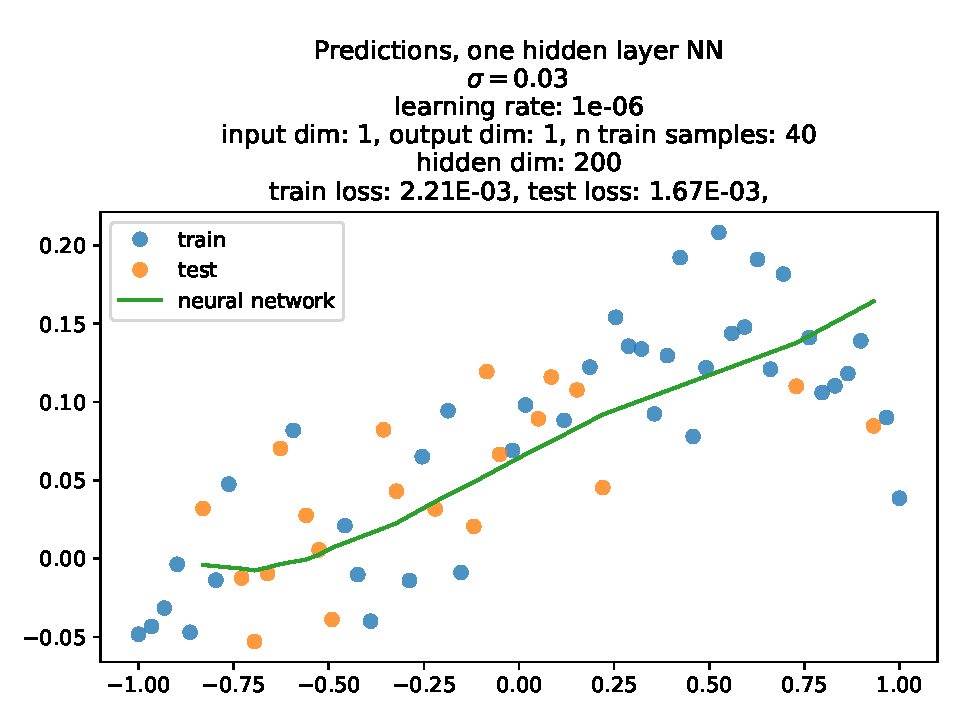
\includegraphics[width=0.8\textwidth]{pred_dim_h_200_lr_1_00E-06}
	\caption{Even with $400$ parameters, this neural network trained with SGD did not overfit !}
	\label{fig:pred_dim_h_200_lr_1_00E-06}
\end{figure}
\end{frame}


\begin{frame}{}
\exercice{}Implement neural network with $1$ hidden layer, with a variable number of hidden neurons, and study the amount of overfitting, also as a function of the learning rate.
\begin{figure}[htpb]
	\centering
	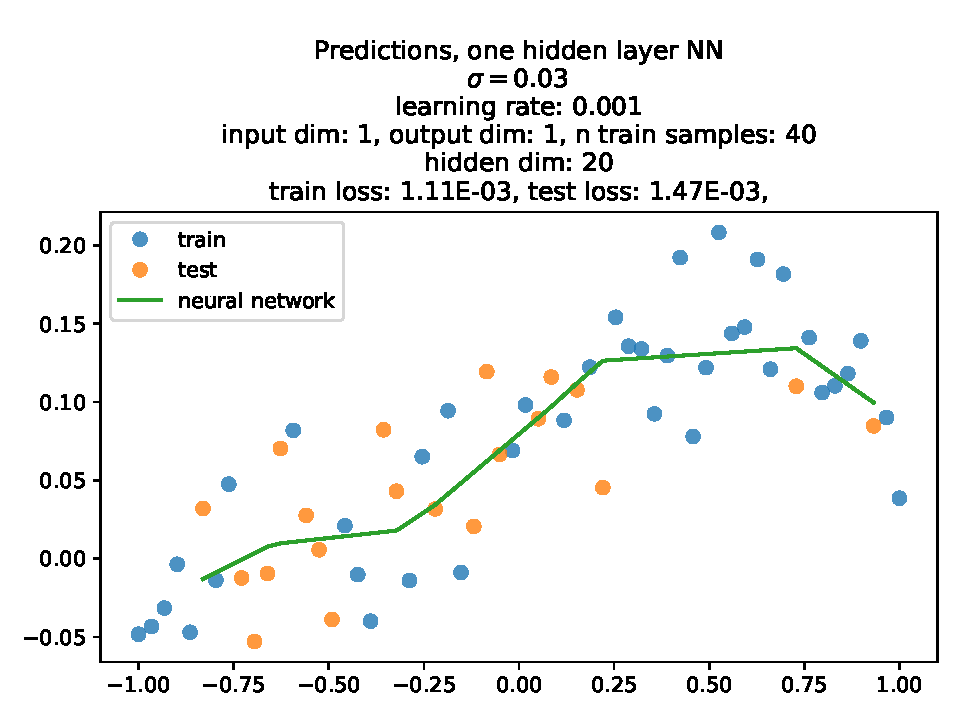
\includegraphics[width=0.6\textwidth]{pred_dim_h_20_lr_1_00E-03}
	\caption{A neural network with $40$ parameters}
	\label{fig:pred_dim_h_200_lr_1_00E-06}
\end{figure}
\end{frame}

\begin{frame}{Learning curves}
\begin{figure}[htpb]
	\centering
	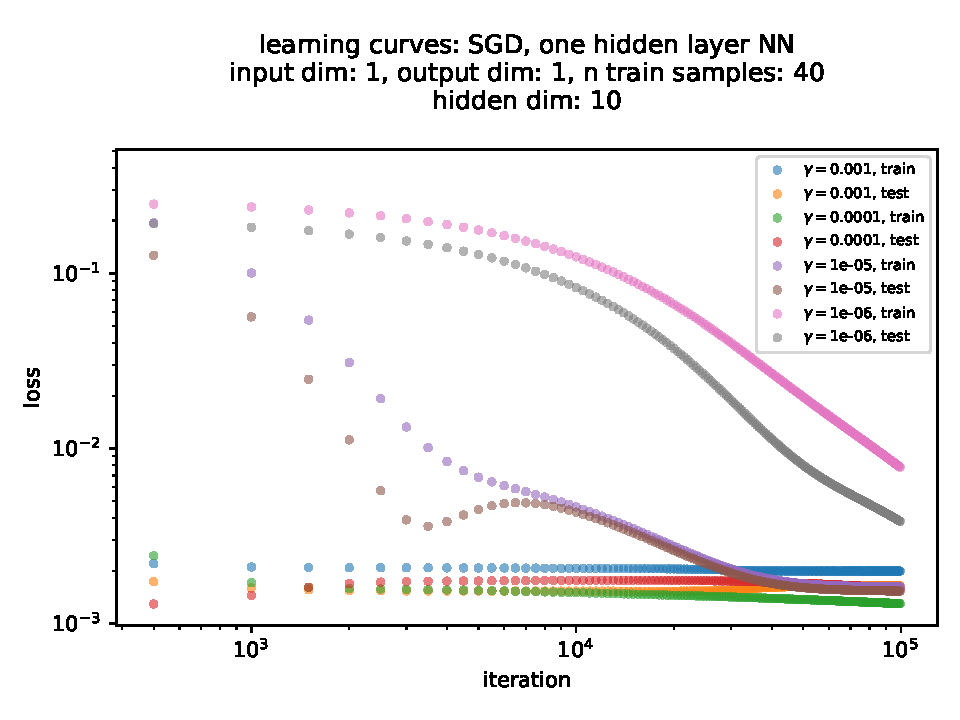
\includegraphics[width=0.8\textwidth]{learning_rates_dim_h_10}
	\label{fig:}
\end{figure}
\end{frame}

\begin{frame}{Learning curves}
\begin{figure}[htpb]
	\centering
	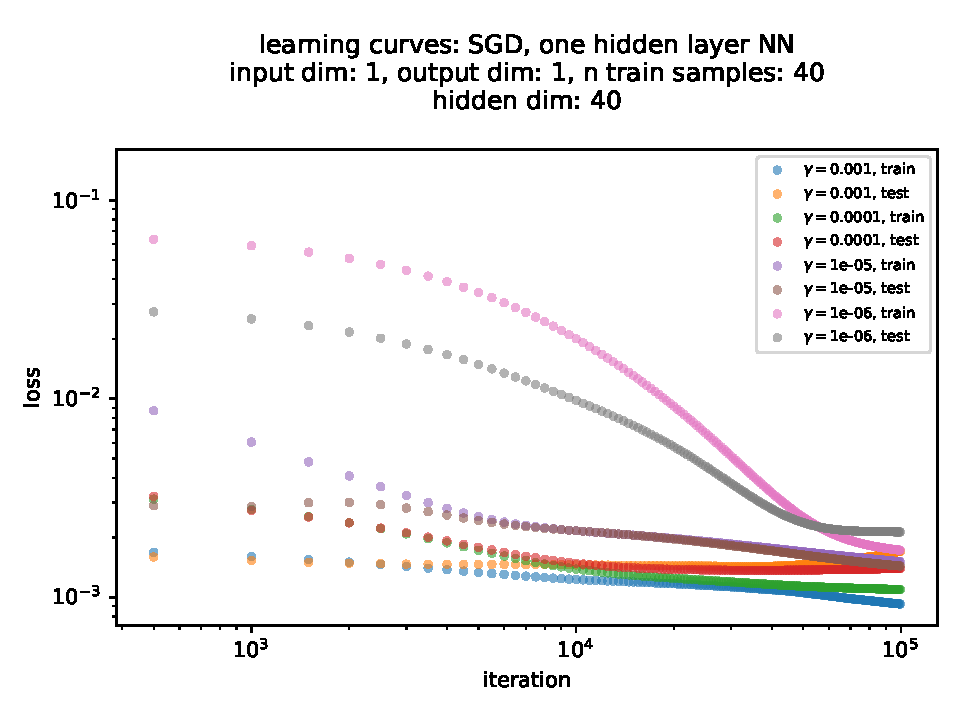
\includegraphics[width=0.8\textwidth]{learning_rates_dim_h_40}
	\label{fig:}
\end{figure}
\end{frame}

\begin{frame}{Learning curves}
\begin{figure}[htpb]
	\centering
	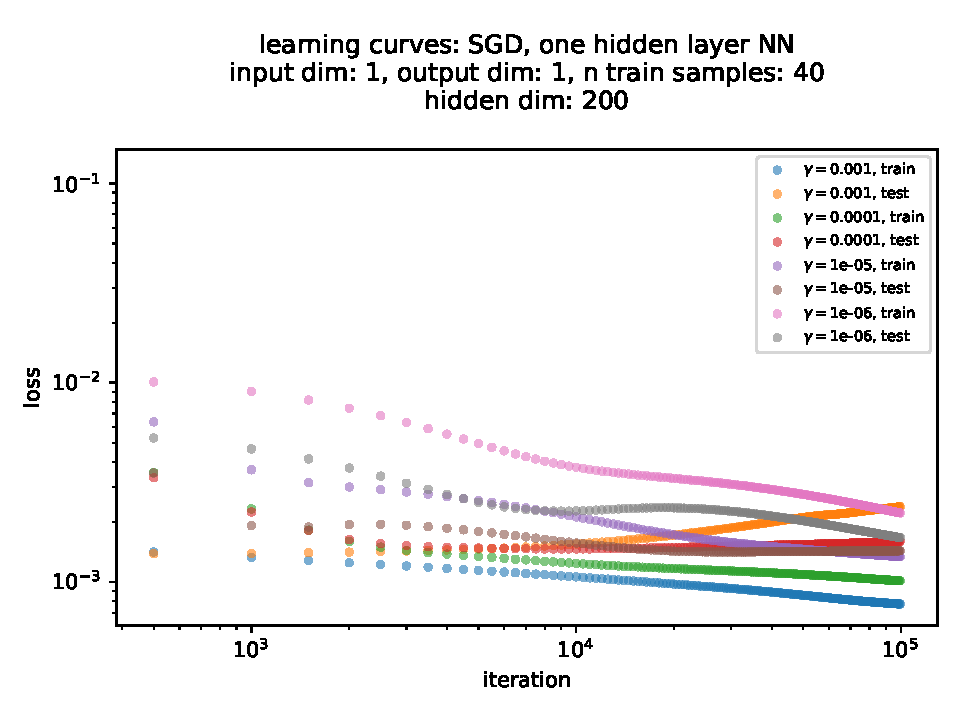
\includegraphics[width=0.8\textwidth]{learning_rates_dim_h_200}
	\label{fig:}
\end{figure}
\end{frame}

% \begin{frame}[allowframebreaks]
% \frametitle{References}
% \bibliographystyle{apalike}
% \bibliography{epita.bib} 
% \end{frame}


\end{document} 
